%!TEX root = ../template.tex
\chapter{State of the art and related work}
\label{cha:state_art}

A sensor is a device that detects or measures a physical property, and converts that value to an electric signal, which is usually transmitted to a processing unit.  

\section{Different Approaches} % (fold)
\label{sec:approaches}
blablablablabla.

\subsection{Video Tracking System Approach}
\label{subsec:video_approach}
blablablablabla.

\subsection{Sensor Tracking System Approach}
\label{subsec:sensor_approach}
blablablablabla.


\section{Sensors} % (fold)
\label{sec:sensors}
blablablablabla.

\subsection{Data Acquisition Sensors in Sports}
\label{subsec:data_sensors}

\subsubsection{Magnetometer}
\label{subsubsec:magnetometer}

\subsection{Motion Sensors}
\label{subsec:motion_sensors}
blablablablabla.

\section{Communication Protocols}
\label{sec:communication_protocols}
blablablablabla.

\subsection{Protocols}
\label{subsec:protocols}

\subsubsection{Cellular}
\label{subsubsec:cellular}
Cellular technology is meant to use cases where the need of data throughput is high, there is a big distance to cover and there are low restraints on power consumption.
Using GSM/3G/4G (and soon 5G), peak data rates can reach up to 20Gbps \cite{5g}. Cellular communication protocol is meant to applications in mobile devices. 

\subsubsection{SigFox}
\label{subsubsec:sigfox}
SigFox builds wireless networks to connect low power objects and devices, which are continuously turned on and send small amounts of data.
SigFox uses Ultra Narrow Band modulation and communicates at 100 or 600 bits per second \cite{sigfox}. 
SigFox is complementary with other technologies, like Bluetooth, GPS, Cellular and WiFi, unleashing the applications of this technology.

\subsubsection{6LoWPAN}
\label{subsubsec:6lowpan}
6LoWPAN comes from the combination of IPv6 and Low Power Wireless Personal Area Network and aims to define the IPv6 to low data rates, low power and small footprint applications, providing an adaptation layer between the MAC and the network layer (IPv6). 
It supports different types of topologies, like star and mesh~\cite{6lowpan}.

\subsubsection{NFC}
\label{subsubsec:nfc}
Near Field Communication is a very short-range (0-10cm) wireless protocol, establishing wireless connections between network appliances and consumer electronic, carrying very low amounts of data (424 Kbits/second).
Some examples are touching the pay terminal with the NFC-enabled phone to authorize the payment, or connecting electronic devices, like a smartphone and a headset~\cite{nfc}.

\subsubsection{ZigBee}
\label{subsubsec:zigbee}

ZigBee is a widely used IoT protocol with different applications in the areas of home automation, offices and healthcare systems.
The networks can be configured in multiple topologies, like star, mesh and cluster tree, and consists in three types of devices: end device, router and coordinator~\cite{protocols}. 

\begin{itemize}
  \item The coordinator is the most capable device, responsible for starting and maintaining the network, store security keys and connect with other networks. 
  \item Router devices can run applications just like de end devices, but additionally can pass information from other devices and extend the network.   
  \item End devices are the simplest and less expensive devices, can only talk to another device, but are able to sleep and to save more power than router or coordinator devices.
\end{itemize}

\subsubsection{Z-Wave}
\label{subsubsec:zwave}

\subsubsection{WiFi}
\label{subsubsec:wifi}

\subsubsection{Bluetooth}
\label{subsubsec:bluetooth}
\begin{table}[ht]
  \caption{Bluetooth Comparison}
  \label{tab:hla:bluetooth_comparison}
  \centering
  \begin{tabular}{lcc}
    \toprule
    \multicolumn{1}{c}{\textbf{Technology}} & \textbf{BR/EDR} & \textbf{BLE} \\
    \midrule
    Setup Time & 100 ms & < 6 ms \\
    Data Rate & 125 Kb/s to 2 Mb/s & 1 Mb/s to 3 Mb/s \\
    Power Consumption & 1 (Reference value) & 0.1 to 0.5 \\
    \bottomrule
  \end{tabular}
  \end{table}

...

Bluetooth network topologies can be of different types, as shown in Figure~\ref{fig:bletopologies}:
\begin{itemize}
\item \textbf{Point-to-point (1:1) -} Point-to-point network topology is used for connecting devices one-to-one. In BR/EDR this type of communication is optimized for audio streaming, like headsets, speakers or free-hands systems. In BLE, this topology is optimized for data transfer with devices like fitness trackers and PC peripherals.
\item \textbf{Broadcast (1:m) -} Broadcast establishes one-to-many connections and is only available in BLE. This topology is optimized for local information sharing, like point-of-interest information, indoor navigation and asset tracking.
\item \textbf{Mesh (m:n) -} Mesh establishes many-to-many device connections and is only available in BLE. This type of topology is useful when a large number of devices are present and need a trustworthy and safe connection network, like a building with automatic lighting functions or a sensor network. Mesh networks can span a very large physical area. This is particularly useful when a device relies on data from another device that is not in his direct range.
\end{itemize}

\begin{figure}[htbp]
    \centering
    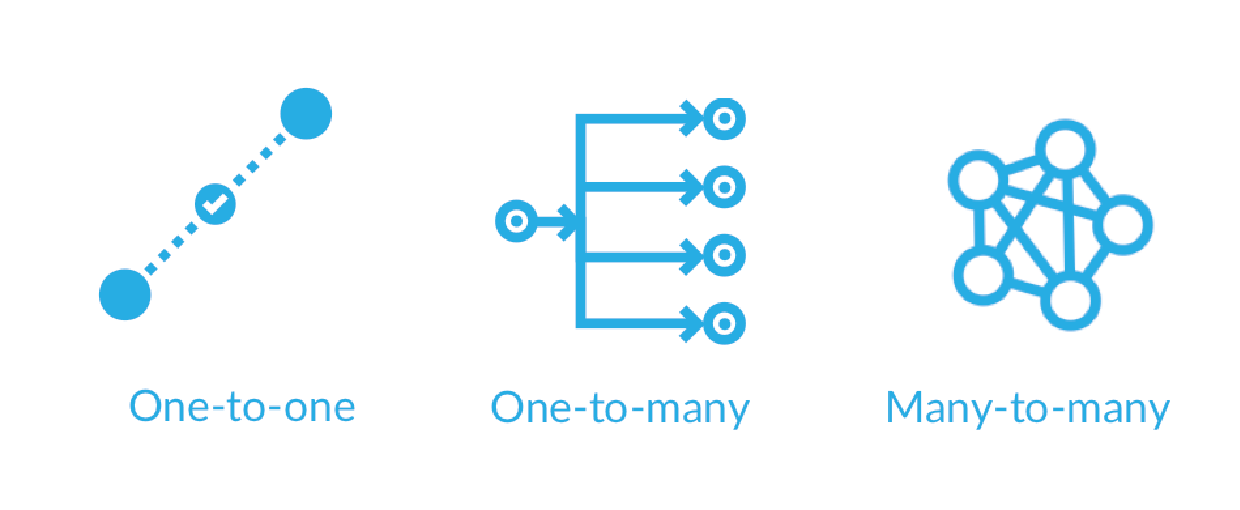
\includegraphics[width=0.5\linewidth]{ble_topologies}
    \caption{BLE Topologies~\cite{ble_mesh_topologies}}
    \label{fig:bletopologies}
\end{figure}


\subsection{Comparison}
\label{subsec:comparison}

As shown in Table \ref{tab:hla:communication_comparison} blablabla

\begin{table}[ht]
\caption{Communication Protocol comparison}
\label{tab:hla:communication_comparison}
\centering
\begin{tabular}{lccccc}
  \toprule
  \multicolumn{1}{c}{\textbf{Technology}} & \textbf{Frequency} & \textbf{Max Data Rate} & \textbf{Range} & \textbf{Power Usage} & \textbf{Cost} \\
  \midrule
  Cellular (4G)                           & Cellular Bands     & 100 Mbps               & Several Km     & High                 & High          \\
  SigFox                                  & < 1 GHz            & < 1 kbps               & Several Km     & Low                  & Medium        \\
  6LoWPAN                                 & < 1 GHz            & 250 kbps               & 100 m          & Low                  & Low           \\
  NFC                                     & 13.56 MHz          & 424 kbps               & 10 cm          & Low                  & Low           \\
  ZigBee                                  & 2.4 GHz            & 250 kbps               & 100 m          & Low                  & Medium        \\
  Z-Wave                                  & < 1 GHz            & 100 kbps               & 30 m           & Low                  & Medium        \\
  WiFi                                    & 2.4/5 GHz          & 54 Mbps                & 100 m          & Medium               & Low           \\
  BLE                                     & 2.4 - 2.48 GHz     & 2 Mbps                 & 100 m          & Low                  & Low           \\

  \bottomrule
\end{tabular}
\end{table}

\section{Related Work} % (fold)
\label{sec:related_work}
The related work was presented in the Section~\ref{sec:approaches}. Camera approaches are the most common system, and provide precise accurate data and can deliver a more interactive experience to fans watching the game, but as presented in Chapter ~\ref{sec:objectives}, they’re against the motivation of this thesis by being costly systems, having the need to be installed in every field where the team plays and because some systems don’t provide real-time data analysis.

The most related works are the sensor-based approaches. Most of these systems include Inertial Measuring Units, but these aren’t used to track the players. Instead, they use other positioning technologies, like GPS in the case of STATSports Apex, Ultra-Wide Band in Kinexon or RFID in Zebra, and use the IMU for gathering information on how the player moves, like counting steps and jumps.

Our system aims to do the tracking and the movement metrics using only the Inertial Measuring Units, without the need of using two systems like most solutions do.


Regarding pedestrian tracking, there are several proposed algorithms to calculate a subject position using IMUs. Carl Fischer, Poorna Sukumar and Mike Hazas propose an approach to implement a tracker using a Kalman Filter and correcting the velocity using zero-velocity updates. 
%[https://ieeexplore.ieee.org/document/6127851]
Sebastian Madgwick presents a novel orientation algorithm, that claims to be more accurate than the Kalman based algorithm. 
%[https://ieeexplore.ieee.org/document/5975346]%
Both approaches use a shoe-mounted sensor.


In the area of activity recognition, there is research in general human activity recognition and in basketball specifically, using inertial measurement units. Kerem Altun and Billur Barshan
%[https://link.springer.com/chapter/10.1007/978-3-642-14715-9_5]
 propose a method to identify several human activities like sitting, standing, walking, climbing stairs and many other, using machine learning techniques. 


Le Nguyen Ngu Nguyen et al. 
%[https://dl.acm.org/citation.cfm?doid=2829875.2829930]%
 use a multi-sensor system to identify general activities like walking, jogging and running, but also basketball-specific activities like jumpshot, layupshot and pivot, using a Support-Vector-Machine-based classifier.

